\documentclass{article}
\usepackage[preprint]{neurips_2025}
\usepackage[utf8]{inputenc}
\usepackage[T1]{fontenc}
\usepackage{hyperref}
\usepackage{url}
\usepackage{booktabs}
\usepackage{amsfonts,amsmath,amssymb}
\usepackage{nicefrac}
\usepackage{microtype}
\usepackage{xcolor}
\usepackage{graphicx}
\usepackage{multirow}
\usepackage{subcaption}

% numbers that are not measured yet are rendered visibly; the final PDF must contain none
\newcommand{\tbd}[1]{\textcolor{red}{[tbd: #1]}}
% generated by bench/make_paper.py -- do not edit
\newcommand{\NSubjectsTotal}{66}
\newcommand{\NEpochsTotal}{36,311}
\newcommand{\NFitsTotal}{818}
\newcommand{\NSeedsMain}{two}
\newcommand{\GPUHours}{95}
\newcommand{\EAMeanDelta}{+0.003}
\newcommand{\EAPosFrac}{26/42}
\newcommand{\EAFMDelta}{+0.004}
\newcommand{\EAScratchDelta}{+0.003}
\newcommand{\BestErrpHriRobot}{0.645}
\newcommand{\BestModelErrpHriRobot}{ErrP-Ens-EA}
\newcommand{\BestRiemannianErrpHriRobot}{0.603}
\newcommand{\BestCompactErrpHriRobot}{0.632}
\newcommand{\BestFoundationErrpHriRobot}{0.597}
\newcommand{\BestOursErrpHriRobot}{0.645}
\newcommand{\BestErrpHriCursor}{0.908}
\newcommand{\BestModelErrpHriCursor}{ErrP-Ens-EA}
\newcommand{\BestRiemannianErrpHriCursor}{0.851}
\newcommand{\BestCompactErrpHriCursor}{0.902}
\newcommand{\BestFoundationErrpHriCursor}{0.891}
\newcommand{\BestOursErrpHriCursor}{0.908}
\newcommand{\BestBnci}{0.871}
\newcommand{\BestModelBnci}{ErrP-Ens}
\newcommand{\BestRiemannianBnci}{0.820}
\newcommand{\BestCompactBnci}{0.849}
\newcommand{\BestFoundationBnci}{0.823}
\newcommand{\BestOursBnci}{0.871}
\newcommand{\BestErpCoreErn}{0.971}
\newcommand{\BestModelErpCoreErn}{ErrP-Ens-EA}
\newcommand{\BestRiemannianErpCoreErn}{0.950}
\newcommand{\BestCompactErpCoreErn}{0.968}
\newcommand{\BestFoundationErpCoreErn}{0.952}
\newcommand{\BestOursErpCoreErn}{0.971}
\newcommand{\BestInterHri}{0.981}
\newcommand{\BestModelInterHri}{ErrP-Ens}
\newcommand{\BestRiemannianInterHri}{0.963}
\newcommand{\BestCompactInterHri}{0.976}
\newcommand{\BestFoundationInterHri}{0.959}
\newcommand{\BestOursInterHri}{0.981}
\newcommand{\CursorMinusRobot}{0.262}
\newcommand{\CursorGtRobot}{12/12}
\newcommand{\CursorRobotP}{5\times10^{-4}}
\newcommand{\FMMinusCompactMean}{-0.021}
\newcommand{\FMWinsDatasets}{0/5}
\newcommand{\EnsMixVsBestMean}{+0.008}
\newcommand{\EnsMixBeatsBest}{5/5}
\newcommand{\EnsMixSigBetter}{0}
\newcommand{\EnsMixSigWorse}{0}
\newcommand{\EnsAllVsBestMean}{+0.004}
\newcommand{\EnsAllBeatsBest}{3/5}
\newcommand{\EnsAllSigBetter}{1}
\newcommand{\EnsAllSigWorse}{0}
\newcommand{\EnsTopVsBestMean}{-0.002}
\newcommand{\EnsTopBeatsBest}{3/5}
\newcommand{\EnsTopSigBetter}{0}
\newcommand{\EnsTopSigWorse}{0}
\newcommand{\EnsMixMeanRank}{1.8}
\newcommand{\EnsMixErrpHriRobot}{0.640}
\newcommand{\EnsMixErrpHriCursor}{0.906}
\newcommand{\EnsMixBnci}{0.871}
\newcommand{\EnsMixErpCoreErn}{0.970}
\newcommand{\EnsMixInterHri}{0.981}
\newcommand{\EnsAllMeanRank}{1.8}
\newcommand{\EnsAllErrpHriRobot}{0.645}
\newcommand{\EnsAllErrpHriCursor}{0.908}
\newcommand{\EnsAllBnci}{0.848}
\newcommand{\EnsAllErpCoreErn}{0.971}
\newcommand{\EnsAllInterHri}{0.974}
\newcommand{\EnsTopMeanRank}{3.8}
\newcommand{\EnsTopErrpHriRobot}{0.640}
\newcommand{\EnsTopErrpHriCursor}{0.905}
\newcommand{\EnsTopBnci}{0.833}
\newcommand{\EnsTopErpCoreErn}{0.969}
\newcommand{\EnsTopInterHri}{0.973}
\newcommand{\BestSingleErrpHriRobot}{0.632}
\newcommand{\BestSingleModelErrpHriRobot}{EEG-Inception + EA}
\newcommand{\BestSingleErrpHriCursor}{0.902}
\newcommand{\BestSingleModelErrpHriCursor}{EEG-Inception + EA}
\newcommand{\BestSingleBnci}{0.849}
\newcommand{\BestSingleModelBnci}{EEG-Inception}
\newcommand{\BestSingleErpCoreErn}{0.968}
\newcommand{\BestSingleModelErpCoreErn}{EEGNeX + EA}
\newcommand{\BestSingleInterHri}{0.976}
\newcommand{\BestSingleModelInterHri}{EEGNeX}
\newcommand{\NVariantsMax}{21}
\newcommand{\EADeltaErrpHriRobot}{+0.021}
\newcommand{\EASigPosErrpHriRobot}{3}
\newcommand{\EASigNegErrpHriRobot}{0}
\newcommand{\EANModelsErrpHriRobot}{8}
\newcommand{\EADeltaErrpHriCursor}{+0.024}
\newcommand{\EASigPosErrpHriCursor}{5}
\newcommand{\EASigNegErrpHriCursor}{0}
\newcommand{\EANModelsErrpHriCursor}{9}
\newcommand{\EADeltaBnci}{-0.023}
\newcommand{\EASigPosBnci}{0}
\newcommand{\EASigNegBnci}{1}
\newcommand{\EANModelsBnci}{8}
\newcommand{\EADeltaErpCoreErn}{+0.006}
\newcommand{\EASigPosErpCoreErn}{3}
\newcommand{\EASigNegErpCoreErn}{0}
\newcommand{\EANModelsErpCoreErn}{8}
\newcommand{\EADeltaInterHri}{-0.012}
\newcommand{\EASigPosInterHri}{0}
\newcommand{\EASigNegInterHri}{3}
\newcommand{\EANModelsInterHri}{9}
\newcommand{\EarlyEEGNetEA}{0.932}
\newcommand{\EarlyEEGNetNone}{0.934}
\newcommand{\EarlyXdawnEA}{0.933}
\newcommand{\EarlyXdawnNone}{0.934}
\newcommand{\RLSeedsText}{10 (FetchReach), 5 (FetchPush), 5 (FetchPush (staged))}
\newcommand{\RLRhoReach}{0.58}
\newcommand{\RLRhoPReach}{2\times10^{-7}}
\newcommand{\RLBreakEvenReach}{0.77}
\newcommand{\RLAUCReachSparse}{0.671}
\newcommand{\RLSuccReachSparse}{0.97}
\newcommand{\RLAUCReachDense}{0.915}
\newcommand{\RLSuccReachDense}{1.00}
\newcommand{\RLGainReachDense}{+0.245}
\newcommand{\RLPosReachDense}{10/10}
\newcommand{\RLSignPReachDense}{0.002}
\newcommand{\RLAUCReachLow}{0.499}
\newcommand{\RLSuccReachLow}{0.92}
\newcommand{\RLGainReachLow}{-0.172}
\newcommand{\RLPosReachLow}{1/10}
\newcommand{\RLSignPReachLow}{0.021}
\newcommand{\RLAUCReachNinety}{0.757}
\newcommand{\RLSuccReachNinety}{0.99}
\newcommand{\RLGainReachNinety}{+0.087}
\newcommand{\RLPosReachNinety}{6/10}
\newcommand{\RLSignPReachNinety}{0.508}
\newcommand{\RLAUCReachExact}{0.800}
\newcommand{\RLSuccReachExact}{0.99}
\newcommand{\RLGainReachExact}{+0.130}
\newcommand{\RLPosReachExact}{9/10}
\newcommand{\RLSignPReachExact}{0.021}
\newcommand{\RLRhoPush}{-0.07}
\newcommand{\RLRhoPPush}{0.695}
\newcommand{\RLBreakEvenPush}{0.75}
\newcommand{\RLAUCPushSparse}{0.045}
\newcommand{\RLSuccPushSparse}{0.04}
\newcommand{\RLAUCPushDense}{0.055}
\newcommand{\RLSuccPushDense}{0.05}
\newcommand{\RLGainPushDense}{+0.009}
\newcommand{\RLPosPushDense}{5/5}
\newcommand{\RLSignPPushDense}{0.062}
\newcommand{\RLAUCPushLow}{0.068}
\newcommand{\RLSuccPushLow}{0.10}
\newcommand{\RLGainPushLow}{+0.022}
\newcommand{\RLPosPushLow}{4/5}
\newcommand{\RLSignPPushLow}{0.375}
\newcommand{\RLAUCPushNinety}{0.046}
\newcommand{\RLSuccPushNinety}{0.04}
\newcommand{\RLGainPushNinety}{+0.001}
\newcommand{\RLPosPushNinety}{2/5}
\newcommand{\RLSignPPushNinety}{1.000}
\newcommand{\RLAUCPushExact}{0.060}
\newcommand{\RLSuccPushExact}{0.09}
\newcommand{\RLGainPushExact}{+0.015}
\newcommand{\RLPosPushExact}{4/5}
\newcommand{\RLSignPPushExact}{0.375}
\newcommand{\RLRhoPushStaged}{0.28}
\newcommand{\RLRhoPPushStaged}{0.103}
\newcommand{\RLBreakEvenPushStaged}{0.55}
\newcommand{\RLAUCPushStagedSparse}{0.045}
\newcommand{\RLSuccPushStagedSparse}{0.04}
\newcommand{\RLAUCPushStagedDense}{0.053}
\newcommand{\RLSuccPushStagedDense}{0.08}
\newcommand{\RLGainPushStagedDense}{+0.008}
\newcommand{\RLPosPushStagedDense}{4/5}
\newcommand{\RLSignPPushStagedDense}{0.375}
\newcommand{\RLAUCPushStagedLow}{0.045}
\newcommand{\RLSuccPushStagedLow}{0.06}
\newcommand{\RLGainPushStagedLow}{-0.001}
\newcommand{\RLPosPushStagedLow}{2/5}
\newcommand{\RLSignPPushStagedLow}{1.000}
\newcommand{\RLAUCPushStagedNinety}{0.056}
\newcommand{\RLSuccPushStagedNinety}{0.13}
\newcommand{\RLGainPushStagedNinety}{+0.011}
\newcommand{\RLPosPushStagedNinety}{3/5}
\newcommand{\RLSignPPushStagedNinety}{1.000}
\newcommand{\RLAUCPushStagedExact}{0.061}
\newcommand{\RLSuccPushStagedExact}{0.06}
\newcommand{\RLGainPushStagedExact}{+0.015}
\newcommand{\RLPosPushStagedExact}{4/5}
\newcommand{\RLSignPPushStagedExact}{0.375}

% fallback for every measured macro: renders a visible [tbd] if the generator did not define it
\providecommand{\BestErrpHriCursor}{\tbd{BestErrpHriCursor}}
\providecommand{\BestErrpHriRobot}{\tbd{BestErrpHriRobot}}
\providecommand{\BestInterHri}{\tbd{BestInterHri}}
\providecommand{\BestModelErrpHriCursor}{\tbd{BestModelErrpHriCursor}}
\providecommand{\BestModelErrpHriRobot}{\tbd{BestModelErrpHriRobot}}
\providecommand{\CursorGtRobot}{\tbd{CursorGtRobot}}
\providecommand{\CursorMinusRobot}{\tbd{CursorMinusRobot}}
\providecommand{\CursorRobotP}{\tbd{CursorRobotP}}
\providecommand{\EADeltaErrpHriCursor}{\tbd{EADeltaErrpHriCursor}}
\providecommand{\EADeltaInterHri}{\tbd{EADeltaInterHri}}
\providecommand{\EAFMDelta}{\tbd{EAFMDelta}}
\providecommand{\EAMeanDelta}{\tbd{EAMeanDelta}}
\providecommand{\EANModelsErrpHriCursor}{\tbd{EANModelsErrpHriCursor}}
\providecommand{\EAPosFrac}{\tbd{EAPosFrac}}
\providecommand{\EarlyEEGNetNone}{\tbd{EarlyEEGNetNone}}
\providecommand{\EarlyXdawnNone}{\tbd{EarlyXdawnNone}}
\providecommand{\EAScratchDelta}{\tbd{EAScratchDelta}}
\providecommand{\EASigNegInterHri}{\tbd{EASigNegInterHri}}
\providecommand{\EASigPosErrpHriCursor}{\tbd{EASigPosErrpHriCursor}}
\providecommand{\EnsAllBeatsBest}{\tbd{EnsAllBeatsBest}}
\providecommand{\EnsAllMeanRank}{\tbd{EnsAllMeanRank}}
\providecommand{\EnsAllSigBetter}{\tbd{EnsAllSigBetter}}
\providecommand{\EnsAllSigWorse}{\tbd{EnsAllSigWorse}}
\providecommand{\EnsAllVsBestMean}{\tbd{EnsAllVsBestMean}}
\providecommand{\EnsTopMeanRank}{\tbd{EnsTopMeanRank}}
\providecommand{\FMMinusCompactMean}{\tbd{FMMinusCompactMean}}
\providecommand{\FMWinsDatasets}{\tbd{FMWinsDatasets}}
\providecommand{\GPUHours}{\tbd{GPUHours}}
\providecommand{\NEpochsTotal}{\tbd{NEpochsTotal}}
\providecommand{\NFitsTotal}{\tbd{NFitsTotal}}
\providecommand{\NSeedsMain}{\tbd{NSeedsMain}}
\providecommand{\NSubjectsTotal}{\tbd{NSubjectsTotal}}
\providecommand{\NVariantsMax}{\tbd{NVariantsMax}}
\providecommand{\RLBreakEvenReach}{\tbd{RLBreakEvenReach}}
\providecommand{\RLRhoPReach}{\tbd{RLRhoPReach}}
\providecommand{\RLRhoReach}{\tbd{RLRhoReach}}
\providecommand{\RLSeedsText}{\tbd{RLSeedsText}}

\title{ErrP-Bench: Do EEG Foundation Models Detect Errors?\\
Benchmarking Error-Related Potential Decoding Across Paradigms\\ and Its Value as Implicit Feedback for Robot Learning}

\author{Anonymous Authors}

\begin{document}
\maketitle

\begin{abstract}
Error-related potentials (ErrPs), the brain's response to observed or committed errors, are a long-standing
candidate for implicit human feedback to robots. Two open questions decide whether this is practical: can
current decoders, including EEG foundation models, detect ErrPs in a new person without calibration, and how
good must such a decoder be before its feedback improves learning? We introduce \textbf{ErrP-Bench}, a
cross-subject benchmark of five public ErrP datasets spanning four error paradigms (\NSubjectsTotal{}
participants, \NEpochsTotal{} epochs), on which we evaluate nine decoders (a Riemannian pipeline, five compact
networks and three pretrained foundation models), each with and without unsupervised per-participant Euclidean
alignment, in \NFitsTotal{} fits. Pretrained models do not outperform compact decoders (best foundation minus
best compact model: \FMMinusCompactMean{} AUROC on average). The observed agent matters more than the decoder:
the same participants yield \BestErrpHriCursor{} AUROC when watching a cursor err and \BestErrpHriRobot{} when
watching a robot err. We then measure a decoder-quality frontier with soft actor-critic on simulated robot
reaching, using feedback of controlled AUROC: the benefit of ErrP reward grows with decoder quality
(Spearman $\rho=\RLRhoReach{}$, $p=\RLRhoPReach{}$) and turns positive only near AUROC \RLBreakEvenReach{}, a
level reached cross-subject by decoders of observed cursor errors but not of observed robot errors. Below it,
ErrP feedback slows learning. Code, prepared-data recipes and per-trial predictions are released.

\end{abstract}

\section{Introduction}
\label{sec:intro}

When a person watches a machine make a mistake, or makes one themselves, the brain produces an
error-related potential (ErrP): a fronto-central negativity followed by a positivity within a few hundred
milliseconds of the error~\citep{chavarriaga2014errare}. Because ErrPs arise without any explicit action,
they have long been proposed as an \emph{implicit} reward signal for teaching robots and
interfaces~\citep{iturrate2015teaching,kim2017intrinsic,salazargomez2017correcting,xu2021accelerating}.
Two developments make this question timely. First, EEG \emph{foundation models} pretrained on thousands of
hours of recordings~\citep{jiang2024labram,wang2024eegpt,wang2025cbramod} promise decoders that transfer
to new people without calibration. Second, learning from human feedback has become a central tool in
machine learning~\citep{christiano2017deep}, and a brain signal would make such feedback free.

Whether either promise holds for ErrPs is unclear. Existing EEG foundation-model benchmarks cover many
paradigms but at most one ErrP dataset~\citep{lu2026omnieegbench,liu2026eegfmcompass}, and ErrP studies typically
evaluate a single dataset with its own protocol. On the RL side, studies of ErrP-based reward report
gains from simulated or near-ideal feedback, but rarely ask how good a \emph{real} cross-subject decoder must
be before its feedback helps.

We address both gaps with \textbf{ErrP-Bench}, a benchmark and measurement study:
\begin{itemize}
\item \textbf{Five ErrP datasets across four error paradigms}: observed robot errors and observed cursor
  errors~\citep{ehrlich2019feasibility}, cursor-monitoring errors~\citep{chavarriaga2010learning},
  self-generated response errors (ERN, flanker task)~\citep{kappenman2021erpcore}, and errors introduced by an
  arm orthosis~\citep{kueper2024eegemg}; \NSubjectsTotal{} participants and \NEpochsTotal{} epochs in total, all
  used in full under one preprocessing and evaluation protocol.
\item \textbf{Nine decoders} from three families: a Riemannian pipeline~\citep{rivet2009xdawn,barachant2012multiclass},
  five compact networks trained from scratch~\citep{lawhern2018eegnet,santamariavazquez2020eeginception,chen2024eegnex,song2023eegconformer,zhao2024ctnet},
  and three pretrained foundation models (LaBraM, EEGPT, CBraMod), each with and without unsupervised
  per-subject Euclidean alignment~\citep{he2020transfer}; \NFitsTotal{} cross-subject fits.
\item \textbf{A decoder-quality frontier for learning from ErrP feedback}: soft actor-critic~\citep{haarnoja2018sac}
  on FetchReach and FetchPush~\citep{plappert2018multigoal} with feedback of controlled AUROC, which locates
  the decoder quality at which ErrP reward starts to help, and places every decoder of the benchmark on it.
\end{itemize}

\textbf{Findings.} \FindingOne{} \FindingTwo{} \FindingThree{}

All code, prepared-data recipes, per-trial predictions and checkpoints are released.

\section{Related work}
\label{sec:related}

\paragraph{Error-related potentials.} The error-related negativity was first described for self-generated
response errors~\citep{falkenstein1991effects,gehring1993neural}; observation and interaction ErrPs follow
erroneous feedback or machine actions~\citep{chavarriaga2010learning,chavarriaga2014errare}. ErrPs have been
decoded to correct robot actions online~\citep{salazargomez2017correcting}, to teach interfaces
\citep{iturrate2015teaching}, and to shape the reward of robot learners~\citep{kim2017intrinsic,akinola2020accelerated,xu2021accelerating}.
Most of these works decode within subjects after a calibration session. Public datasets now span visual
observation~\citep{ehrlich2019feasibility,chavarriaga2010learning}, self-generated
errors~\citep{kappenman2021erpcore} and physically introduced errors~\citep{kueper2024eegemg,chari2024interhri},
but no common cross-subject protocol compares them.

\paragraph{EEG decoders and foundation models.} Compact convolutional networks such as
EEGNet~\citep{lawhern2018eegnet} and EEG-Inception~\citep{santamariavazquez2020eeginception}, convolution-transformer
hybrids~\citep{song2023eegconformer,zhao2024ctnet,chen2024eegnex}, and Riemannian pipelines built on xDAWN
spatial filtering~\citep{rivet2009xdawn,barachant2012multiclass} are standard for event-related potentials.
Foundation models pretrain transformers on large unlabeled corpora and fine-tune on the target task:
LaBraM~\citep{jiang2024labram}, EEGPT~\citep{wang2024eegpt} and CBraMod~\citep{wang2025cbramod} are the
open models we evaluate. Cross-subject shift is also addressed without labels by aligning each subject's
data, e.g.\ Euclidean alignment~\citep{he2020transfer} or Riemannian re-centering~\citep{zanini2018transfer}.

\paragraph{Benchmarks.} MOABB~\citep{jayaram2018moabb,chevallier2024moabbbenchmark} standardised classical BCI paradigms;
recent foundation-model benchmarks evaluate many tasks and report mixed gains over specialist
models~\citep{kastrati2025eegbench,lu2026omnieegbench,liu2026eegfmcompass,kokate2026channel}. ErrPs appear there as one task
among dozens. ErrP-Bench is complementary: it covers the error paradigms in depth, tests whether
alignment or pretraining matters more, and measures the downstream value of the decoded signal for learning.

\section{ErrP-Bench}
\label{sec:bench}

\subsection{Datasets}
Table~\ref{tab:datasets} lists the five dataset conditions. All are public and used in full: every
participant and every recording of the paradigm. Labels come from each dataset's own event documentation.

\begin{table}[t]
\centering
\caption{ErrP-Bench datasets. ``Error'' is the label-1 class; epochs are time-locked to the error-eliciting
event (feedback, machine action, response or orthosis perturbation).}
\label{tab:datasets}
\small
\resizebox{\linewidth}{!}{\begin{tabular}{llrrrrrl}
\toprule
Dataset & Paradigm & Subj. & Ch. & Epochs & Error \% & Min err./subj. & Window (s) \\
\midrule
ErrP-HRI robot & observed robot error & 12 & 27 & 5,822 & 35.3 & 155 & [0.0, 2.0) \\
ErrP-HRI cursor & observed cursor error & 12 & 27 & 5,806 & 34.2 & 153 & [0.0, 2.0) \\
BNCI 2015-013 & cursor monitoring & 6 & 64 & 6,437 & 20.5 & 188 & [0.0, 1.0) \\
ERP CORE ERN & own response error (flanker) & 40 & 28 & 15,756 & 10.6 & 2 & [-0.2, 0.8) \\
IntEr-HRI & orthosis-introduced error & 8 & 65 & 2,490 & 20.0 & 60 & [0.0, 1.0) \\
\bottomrule
\end{tabular}
}
\end{table}

\textbf{ErrP-HRI}~\citep{ehrlich2019feasibility}: participants watch a robot (\emph{robot}) or a cursor
(\emph{cursor}) execute a direction they selected; in machine-error trials the executed movement differs from the
selected one. 12 participants per condition, 27 channels, mastoid reference. We use both conditions as separate
datasets, so that the effect of the observed agent is measured with the participants held fixed.
\textbf{BNCI 2015-013}~\citep{chavarriaga2010learning}: participants monitor a cursor that moves toward a target
and errs in about 20\% of steps. \textbf{ERP CORE ERN}~\citep{kappenman2021erpcore}: 40 participants perform a
flanker task; epochs are locked to the participant's own response, incorrect responses are errors.
\textbf{IntEr-HRI}~\citep{kueper2024eegemg,chari2024interhri}: an active orthosis moves the participant's arm
and in some trials briefly reverses (error); correct events are the authors' matched mid-movement markers.
Participants squeezed a ball when they noticed an error; in about 90\% of error epochs the squeeze falls inside
the window (median 0.72\,s after the error), so this dataset measures an error-plus-response signal; we report a
control restricted to the first 0.5\,s.

\textbf{Preprocessing} is identical in kind across datasets: scalp channels only, zero-phase FIR band-pass
1--20\,Hz~\citep{gramfort2013mne} on the continuous recording, epochs of whole seconds after the event (2\,s for
ErrP-HRI, the window used in its original analysis; 1\,s otherwise), resampling to 256\,Hz (Riemannian and compact models), 200\,Hz (LaBraM, CBraMod) or 250\,Hz (EEGPT), the rates
the foundation models were pretrained at, no amplitude-based rejection. Channel names follow the 10--20 system so that
channel-aware foundation models receive their own position embeddings.

\subsection{Protocol}
\textbf{Cross-subject} evaluation is the primary protocol, since an implicit feedback signal is useful only if it
works for a new person without a calibration session. Participants of a dataset are split into five disjoint
test groups; in each fold, about 15\% of the remaining participants form a validation set that is used only for
early stopping, and the rest are training participants. Every participant is tested exactly once. The unit of
analysis is the held-out participant: we report the macro average over participants of the per-participant
AUROC, averaged over training seeds (\NSeedsMain{} seeds per configuration). AUROC is threshold-free and robust to
the class imbalance of ErrP data. Differences between decoders are tested with two-sided Wilcoxon signed-rank
tests over participants, Holm-corrected within each dataset~\citep{demsar2006statistical}.

\subsection{Training protocol}
The decoders of Table~\ref{tab:decoders} are trained on the training participants of each fold.
Networks trained from scratch use their braindecode implementations~\citep{schirrmeister2017deep}, Adam,
at most 150 epochs and early stopping with patience 20. Foundation models are initialised from their released
pretrained weights and fully fine-tuned with a new classification head (backbone learning rate $10^{-4}$, head
$5\times10^{-4}$, AdamW, cosine schedule, at most 30 epochs, patience 10). All networks use class-weighted
cross-entropy (Eq.~\ref{eq:loss}) and select the checkpoint with the best validation AUROC. Hyperparameters are
the published defaults; no decoder receives dataset-specific tuning, so every decoder has the same tuning budget.
Every decoder is trained with and without Euclidean alignment (Eq.~\ref{eq:ea}), with two training seeds
(xDAWN is deterministic and run once; EEGPT, the most expensive model, with one seed). ErrP-Ens requires no
training: it combines the saved test predictions of the members (Eq.~\ref{eq:ens}).

\section{Decoding results}
\label{sec:results}

\begin{table}[t]
\centering
\caption{Cross-subject decoding on ErrP-Bench: macro-participant AUROC (mean $\pm$ SD over training seeds;
$^{\ast}$: one seed). Bold: best per dataset. Rank: mean rank over datasets ($^{\dagger}$: not run on every
dataset). EA: per-participant Euclidean alignment. Pairwise tests of the best decoder against every other are
in Appendix~\ref{app:stats}.}
\label{tab:main}
\scriptsize
\setlength{\tabcolsep}{3pt}
\resizebox{\linewidth}{!}{\begin{tabular}{lllcccccc}
\toprule
Family & Model & EA & ErrP-HRI robot & ErrP-HRI cursor & BNCI 2015-013 & ERP CORE ERN & IntEr-HRI & Rank \\
\midrule
Riemannian & xDAWN+RG &  & 0.590\scriptsize{$^{\ast}$} & 0.823\scriptsize{$^{\ast}$} & 0.820\scriptsize{$^{\ast}$} & 0.945\scriptsize{$^{\ast}$} & 0.955\scriptsize{$^{\ast}$} & 15.6 \\
Riemannian & xDAWN+RG & \checkmark & 0.603\scriptsize{$^{\ast}$} & 0.851\scriptsize{$^{\ast}$} & 0.803\scriptsize{$^{\ast}$} & 0.950\scriptsize{$^{\ast}$} & 0.963\scriptsize{$^{\ast}$} & 13.4 \\
\midrule
compact & EEGNet &  & 0.570\scriptsize{$\pm$0.008} & 0.872\scriptsize{$\pm$0.002} & 0.823\scriptsize{$^{\ast}$} & 0.959\scriptsize{$\pm$0.002} & 0.974\scriptsize{$\pm$0.000} & 10.0 \\
compact & EEGNet & \checkmark & 0.606\scriptsize{$\pm$0.004} & 0.885\scriptsize{$\pm$0.006} & 0.803\scriptsize{$\pm$0.002} & 0.963\scriptsize{$\pm$0.000} & 0.947\scriptsize{$\pm$0.006} & 11.2 \\
compact & EEG-Inception &  & 0.591\scriptsize{$\pm$0.000} & 0.873\scriptsize{$\pm$0.011} & 0.849\scriptsize{$\pm$0.005} & 0.958\scriptsize{$\pm$0.002} & 0.970\scriptsize{$\pm$0.002} & 9.2 \\
compact & EEG-Inception & \checkmark & 0.632\scriptsize{$\pm$0.013} & 0.902\scriptsize{$\pm$0.002} & 0.809\scriptsize{$\pm$0.003} & 0.966\scriptsize{$\pm$0.001} & 0.967\scriptsize{$\pm$0.002} & 7.2 \\
compact & EEGNeX &  & 0.623\scriptsize{$\pm$0.000} & 0.878\scriptsize{$\pm$0.010} & 0.841\scriptsize{$\pm$0.001} & 0.963\scriptsize{$\pm$0.002} & 0.976\scriptsize{$\pm$0.003} & 5.8 \\
compact & EEGNeX & \checkmark & 0.622\scriptsize{$\pm$0.014} & 0.897\scriptsize{$\pm$0.005} & 0.809\scriptsize{$\pm$0.013} & 0.968\scriptsize{$\pm$0.000} & 0.971\scriptsize{$\pm$0.004} & 7.2 \\
compact & EEG-Conformer &  & 0.594\scriptsize{$\pm$0.004} & 0.792\scriptsize{$\pm$0.009} & 0.820\scriptsize{$\pm$0.003} & 0.950\scriptsize{$\pm$0.001} & 0.964\scriptsize{$\pm$0.004} & 14.0 \\
compact & EEG-Conformer & \checkmark & 0.597\scriptsize{$\pm$0.002} & 0.840\scriptsize{$\pm$0.001} & 0.788\scriptsize{$\pm$0.000} & 0.953\scriptsize{$\pm$0.002} & 0.960\scriptsize{$\pm$0.002} & 14.2 \\
compact & CTNet &  & 0.596\scriptsize{$\pm$0.016} & 0.873\scriptsize{$\pm$0.004} & 0.846\scriptsize{$\pm$0.023} & 0.959\scriptsize{$\pm$0.001} & 0.954\scriptsize{$\pm$0.000} & 10.8 \\
compact & CTNet & \checkmark & 0.617\scriptsize{$\pm$0.003} & 0.885\scriptsize{$\pm$0.005} & 0.820\scriptsize{$\pm$0.009} & 0.961\scriptsize{$\pm$0.002} & 0.944\scriptsize{$\pm$0.006} & 10.4 \\
\midrule
foundation & LaBraM &  & 0.554\scriptsize{$\pm$0.001} & 0.824\scriptsize{$\pm$0.002} & 0.801\scriptsize{$\pm$0.010} & 0.944\scriptsize{$\pm$0.001} & 0.955\scriptsize{$\pm$0.007} & 18.0 \\
foundation & LaBraM & \checkmark & 0.564\scriptsize{$\pm$0.002} & 0.851\scriptsize{$\pm$0.015} & 0.779\scriptsize{$\pm$0.014} & 0.952\scriptsize{$\pm$0.006} & 0.953\scriptsize{$\pm$0.007} & 16.8 \\
foundation & EEGPT &  & 0.582\scriptsize{$^{\ast}$} & 0.854\scriptsize{$^{\ast}$} & 0.812\scriptsize{$^{\ast}$} & -- & 0.957\scriptsize{$^{\ast}$} & 14.0$^{\dagger}$ \\
foundation & EEGPT & \checkmark & 0.623\scriptsize{$^{\ast}$} & 0.891\scriptsize{$^{\ast}$} & 0.778\scriptsize{$^{\ast}$} & -- & 0.920\scriptsize{$^{\ast}$} & 13.2$^{\dagger}$ \\
foundation & CBraMod &  & 0.554\scriptsize{$\pm$0.008} & 0.838\scriptsize{$\pm$0.004} & 0.819\scriptsize{$\pm$0.017} & 0.944\scriptsize{$\pm$0.002} & 0.959\scriptsize{$\pm$0.005} & 16.2 \\
foundation & CBraMod & \checkmark & 0.597\scriptsize{$\pm$0.001} & 0.845\scriptsize{$\pm$0.009} & 0.823\scriptsize{$\pm$0.002} & 0.952\scriptsize{$\pm$0.000} & 0.930\scriptsize{$\pm$0.006} & 13.8 \\
\midrule
ours & ErrP-Ens & both & 0.642\scriptsize{$\pm$0.003} & 0.906\scriptsize{$\pm$0.002} & \textbf{0.872\scriptsize{$\pm$0.004}} & 0.970\scriptsize{$\pm$0.001} & \textbf{0.981\scriptsize{$\pm$0.001}} & 1.6 \\
ours & ErrP-Ens-EA & \checkmark & \textbf{0.649\scriptsize{$\pm$0.001}} & \textbf{0.908\scriptsize{$\pm$0.003}} & 0.851\scriptsize{$\pm$0.002} & \textbf{0.971\scriptsize{$\pm$0.001}} & 0.974\scriptsize{$\pm$0.002} & 1.6 \\
ours & ErrP-Ens-EA (top-3) & \checkmark & 0.640\scriptsize{$\pm$0.008} & 0.905\scriptsize{$\pm$0.001} & 0.833\scriptsize{$\pm$0.001} & 0.969\scriptsize{$\pm$0.000} & 0.973\scriptsize{$\pm$0.001} & 4.0 \\
\bottomrule
\end{tabular}
}
\end{table}

Table~\ref{tab:main} reports every decoder on every dataset. Four results stand out.

\paragraph{The observed agent dominates decoder choice.} The same twelve participants watched both a robot and a
cursor commit the same kind of error. The best cross-subject decoder reaches \BestErrpHriCursor{} AUROC
(\BestModelErrpHriCursor{}) on cursor errors but only \BestErrpHriRobot{} (\BestModelErrpHriRobot{}) on robot
errors. Paired over participants, the cursor condition is higher by \CursorMinusRobot{} for \CursorGtRobot{}
participants (Wilcoxon $p=\CursorRobotP{}$). No decoder, pretrained or not, closes this gap: the
difference between the two conditions is larger than the spread of all nine decoders on either of them. A plausible
reason, which we do not test, is that a robot movement unfolds over time, so the moment at which it becomes an
error is less sharply defined than a cursor jump and the time-locked potential is smeared. For human--robot interaction, this is the
condition that matters, and it is the hardest one in the benchmark.

\paragraph{Pretraining does not buy cross-subject ErrP decoding.} The best foundation model minus the best
compact model averages \FMMinusCompactMean{} AUROC over datasets, and a foundation model is best on
\FMWinsDatasets{} datasets (per-dataset paired tests in Appendix~\ref{app:stats}). On ErrP-HRI robot,
LaBraM and CBraMod are among the weakest decoders. The decoders that do best are small and strongly
inductive: the Riemannian xDAWN pipeline, which needs seconds of CPU time, and EEGNet-style networks. One
interpretation is that ErrPs are low-dimensional, time-locked waveforms: a model that already encodes spatial
filtering and a short temporal template has little left to gain from generic pretraining, whereas a large
backbone fine-tuned on a few thousand trials from about ten participants can fit the training participants
too closely.

\paragraph{Unsupervised alignment helps when the paradigm is consistent.} EA changes AUROC by \EAMeanDelta{} on
average over all model--dataset pairs, improving \EAPosFrac{} of them (Table~\ref{tab:ea}). Its effect depends
on the dataset: \EADeltaErrpHriCursor{} on ErrP-HRI cursor (\EASigPosErrpHriCursor{} of \EANModelsErrpHriCursor{}
models significantly better) but \EADeltaInterHri{} on IntEr-HRI (\EASigNegInterHri{} significantly worse).
EA removes between-participant differences in spatial covariance; our hypothesis for the negative cases is that
when that covariance is shaped by the task itself (in IntEr-HRI, the arm movement and the ball squeeze),
whitening it also removes signal. The averages over families are \EAScratchDelta{} for networks trained from scratch and \EAFMDelta{}
for foundation models.

\paragraph{Label-free ensembling.} ErrP-Ens averages, per participant, the within-participant ranks of the
aligned decoders. It needs no labels from the new participant and no training. Its mean rank over datasets is
\EnsAllMeanRank{} (all members) and \EnsTopMeanRank{} (validation top-3), among up to \NVariantsMax{} variants.
Against the best single decoder of each dataset (chosen with hindsight on the test participants, so the
comparison favours the single model), ErrP-Ens (all) differs by \EnsAllVsBestMean{} on average, is higher on
\EnsAllBeatsBest{} datasets, and is significantly better on \EnsAllSigBetter{} and significantly worse on
\EnsAllSigWorse{} after Holm correction.

\begin{table}[t]
\centering
\caption{Effect of Euclidean alignment: AUROC with EA minus without, averaged over seeds and participants.
$^{\ast}$: paired Wilcoxon $p<0.05$ over participants (uncorrected).}
\label{tab:ea}
\scriptsize
\resizebox{\linewidth}{!}{\begin{tabular}{lcccccc}
\toprule
Model & ErrP-HRI robot & ErrP-HRI cursor & BNCI 2015-013 & ERP CORE ERN & IntEr-HRI & Mean $\Delta$ \\
\midrule
xDAWN+RG & +0.013 & +0.028$^{\ast}$ & -0.017 & +0.006 & +0.008 & +0.007 \\
EEGNet & +0.036$^{\ast}$ & +0.013 & -0.020 & +0.005$^{\ast}$ & -0.027$^{\ast}$ & +0.002 \\
EEG-Inception & +0.041 & +0.028$^{\ast}$ & -0.041$^{\ast}$ & +0.009$^{\ast}$ & -0.003 & +0.007 \\
EEGNeX & -0.001 & +0.018 & -0.033 & +0.006$^{\ast}$ & -0.005 & -0.003 \\
EEG-Conformer & +0.002 & +0.048$^{\ast}$ & -0.032 & +0.002 & -0.004 & +0.004 \\
CTNet & +0.021$^{\ast}$ & +0.012 & -0.026 & +0.003 & -0.010 & +0.000 \\
LaBraM & +0.009 & +0.026$^{\ast}$ & -0.021 & +0.008 & -0.002 & +0.004 \\
EEGPT & +0.041$^{\ast}$ & +0.037$^{\ast}$ & -0.034 & -- & -0.037$^{\ast}$ & +0.002 \\
CBraMod & +0.043$^{\ast}$ & +0.007 & +0.004 & +0.007 & -0.029$^{\ast}$ & +0.006 \\
\bottomrule
\end{tabular}
}
\end{table}

\paragraph{IntEr-HRI measures more than an ErrP.} Decoders reach AUROC near \BestInterHri{} on IntEr-HRI. In
about 90\% of its error epochs the participant's ball squeeze, a motor response to the error, falls inside the
window. Restricted to the first 0.5\,s, before almost all squeezes (0.8\% occur earlier), EEGNet still reaches
\EarlyEEGNetNone{} and xDAWN \EarlyXdawnNone{}. A large part of the discriminative signal therefore precedes
the squeeze, but the full-window scores should be read as an upper bound for an error-plus-response signal.

\section{How good must an error decoder be? A decoder-quality frontier for learning}
\label{sec:rl}

Decoding accuracy is a proxy. The quantity that matters for implicit feedback is whether a learner improves
when its reward includes the decoded error probability. We measure this directly, as a function of decoder
quality, with real reinforcement learning.

\paragraph{Setup.} Soft actor-critic (Stable-Baselines3~\citep{raffin2021sb3}) learns FetchReach and FetchPush
(Gymnasium-Robotics~\citep{delazcano2024gymnasiumrobotics}, MuJoCo~\citep{todorov2012mujoco}) with the reward of
Eq.~\ref{eq:reward}; the distance that labels segments is gripper--goal for Reach and object--goal for Push.
The ErrP decoder is replaced by feedback of controlled AUROC (Eq.~\ref{eq:binormal}; see also
\citet{hanley1982meaning}) at levels 0.55, 0.60, 0.65, 0.70, 0.80, 0.90 and 1.0 (exact labels), with sparse and
dense ($10\times$ distance decrease) reward as references. Budgets are 150k environment steps (Reach) and 500k
(Push); every 10k steps the deterministic policy is evaluated on 100 fixed held-out goals with the sparse success
criterion. Learning speed, the normalised area under this success curve, is the primary metric, because final
success saturates on Reach. Seeds per condition: \RLSeedsText{}. Because the object rarely moves early in
FetchPush, the object--goal rule yields little feedback there; a supplementary \emph{staged} variant labels
segments by the change in gripper--object plus object--goal distance (its sparse reference is the same sparse
run, since the rule does not affect sparse training).

\paragraph{Results.} On FetchReach (Figure~\ref{fig:frontier}, Table~\ref{tab:rl}), the benefit of ErrP feedback rises
monotonically with decoder quality: across all runs, the paired gain in normalized success AUC over the sparse
run of the same seed is rank-correlated with feedback AUROC (Spearman $\rho=\RLRhoReach{}$, $p=\RLRhoPReach{}$).
Exact feedback raises the AUC from \RLAUCReachSparse{} to \RLAUCReachExact{} (\RLPosReachExact{} seeds better,
sign test $p=\RLSignPReachExact{}$), about half of the gain of the dense reward (\RLAUCReachDense{}). The mean gain
crosses zero at AUROC \RLBreakEvenReach{} (linear interpolation between the measured levels). Below this point the
feedback is harmful: at AUROC 0.55 the AUC drops to \RLAUCReachLow{} (\RLGainReachLow{}, \RLPosReachLow{} seeds
better, $p=\RLSignPReachLow{}$). Final success saturates for every condition (at least \RLSuccReachLow{}), so the
effect is on learning speed. Noisy feedback is therefore not merely uninformative; a likely reason is that, with a
fixed weight, it adds a reward term that is only weakly correlated with progress and that the critic must
fit nonetheless.

On FetchPush, SAC without hindsight relabelling does not learn the task within 500k steps in any condition
(final success \RLSuccPushSparse{} with sparse reward, \RLSuccPushDense{} with dense reward,
\RLSuccPushExact{} with exact ErrP feedback), and no condition differs reliably from sparse. Push therefore shows
that ErrP feedback of any quality does not substitute for exploration when the learner rarely moves the object;
it does not locate a frontier. The staged label rule, which provides several times more feedback events, gives
the same picture (Table~\ref{tab:rl}, right).

Placing the benchmark on the Reach frontier (vertical lines in Figure~\ref{fig:frontier}): the best
cross-subject decoders of cursor errors, cursor-monitoring errors, response errors and orthosis errors lie above
the break-even point, whereas the best decoder of observed robot errors (\BestErrpHriRobot{}) lies well below
it, in the range where feedback slowed learning.


\begin{figure}[t]
\centering
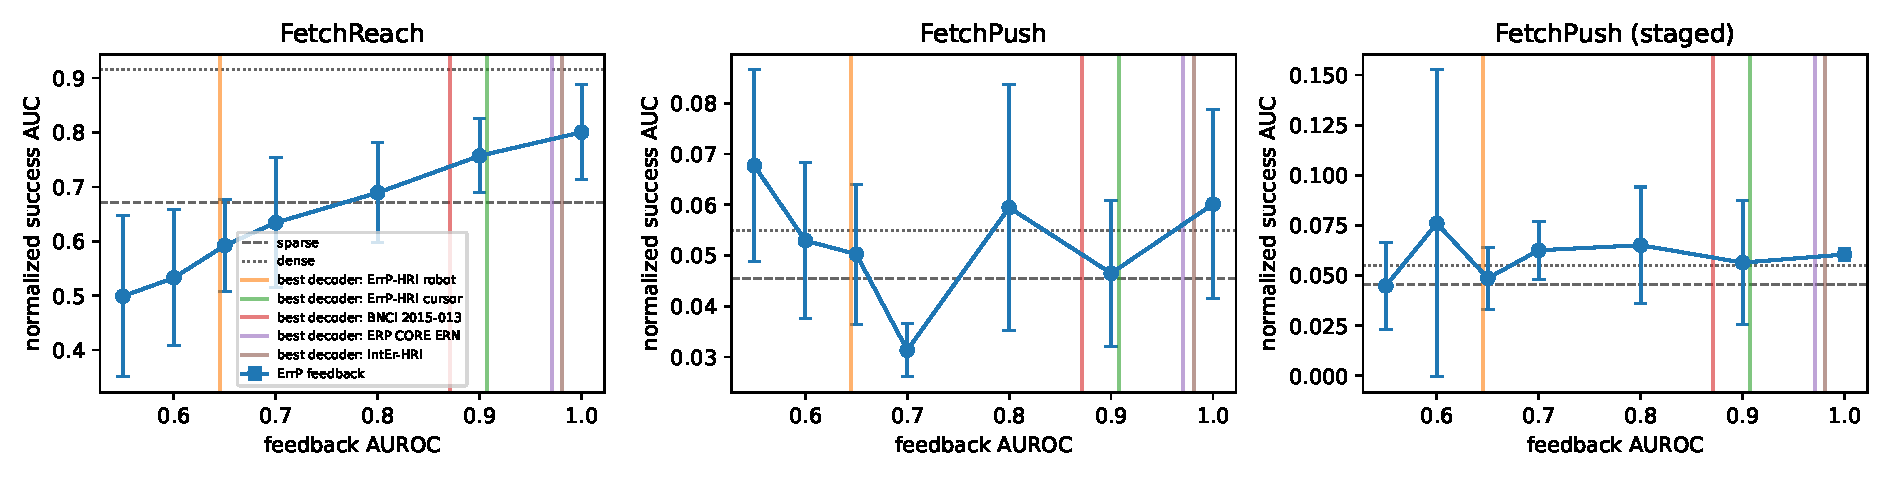
\includegraphics[width=\linewidth]{figures/frontier.pdf}
\caption{Decoder-quality frontier. Normalized success AUC (mean $\pm$ SD over five seeds) of SAC with ErrP
feedback of controlled AUROC; horizontal lines: sparse and dense reward. Vertical lines: the cross-subject AUROC
of the best ErrP-Bench decoder on each dataset.}
\label{fig:frontier}
\end{figure}

\begin{figure}[t]
\centering
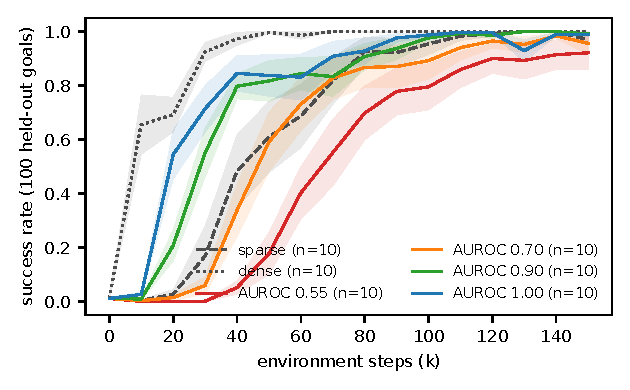
\includegraphics[width=0.62\linewidth]{figures/rl_curves.pdf}
\caption{FetchReach learning curves (success on 100 held-out goals; mean $\pm$ s.e.m. over 10 seeds) for sparse
and dense reward and for ErrP feedback of four quality levels. Low-quality feedback delays learning relative to
the sparse reward; high-quality feedback accelerates it.}
\label{fig:rlcurves}
\end{figure}

\begin{table}[t]
\centering
\caption{Normalized success AUC (mean $\pm$ SD over seeds) and its paired difference to the sparse-reward run of
the same seed ($k/n$: seeds with a positive difference).}
\label{tab:rl}
\scriptsize
\resizebox{\linewidth}{!}{\begin{tabular}{lcccccc}
\toprule
Feedback & \multicolumn{2}{c}{FetchReach} & \multicolumn{2}{c}{FetchPush} & \multicolumn{2}{c}{FetchPush (staged)} \\
 & norm.\ AUC & $\Delta$ vs sparse & norm.\ AUC & $\Delta$ vs sparse & norm.\ AUC & $\Delta$ vs sparse \\
\midrule
sparse only & 0.671\scriptsize{$\pm$0.106} & ref & 0.045\scriptsize{$\pm$0.011} & ref & 0.045\scriptsize{$\pm$0.011} & ref \\
dense (reference) & 0.915\scriptsize{$\pm$0.029} & +0.245 (10/10) & 0.055\scriptsize{$\pm$0.007} & +0.009 (5/5) & 0.053\scriptsize{$\pm$0.015} & +0.008 (4/5) \\
AUROC 0.55 & 0.499\scriptsize{$\pm$0.148} & -0.172 (1/10) & 0.068\scriptsize{$\pm$0.019} & +0.022 (4/5) & 0.045\scriptsize{$\pm$0.022} & -0.001 (2/5) \\
AUROC 0.60 & 0.533\scriptsize{$\pm$0.125} & -0.138 (2/10) & 0.053\scriptsize{$\pm$0.015} & +0.007 (4/5) & 0.076\scriptsize{$\pm$0.077} & +0.031 (3/5) \\
AUROC 0.65 & 0.592\scriptsize{$\pm$0.084} & -0.078 (1/10) & 0.050\scriptsize{$\pm$0.014} & +0.005 (4/5) & 0.049\scriptsize{$\pm$0.015} & +0.003 (3/5) \\
AUROC 0.70 & 0.634\scriptsize{$\pm$0.120} & -0.036 (5/10) & 0.031\scriptsize{$\pm$0.005} & -0.014 (0/5) & 0.063\scriptsize{$\pm$0.014} & +0.017 (5/5) \\
AUROC 0.80 & 0.689\scriptsize{$\pm$0.092} & +0.019 (5/10) & 0.059\scriptsize{$\pm$0.024} & +0.014 (4/5) & 0.065\scriptsize{$\pm$0.029} & +0.020 (4/5) \\
AUROC 0.90 & 0.757\scriptsize{$\pm$0.068} & +0.087 (6/10) & 0.046\scriptsize{$\pm$0.014} & +0.001 (2/5) & 0.056\scriptsize{$\pm$0.031} & +0.011 (3/5) \\
AUROC 1.00 (exact) & 0.800\scriptsize{$\pm$0.087} & +0.130 (9/10) & 0.060\scriptsize{$\pm$0.019} & +0.015 (4/5) & 0.061\scriptsize{$\pm$0.003} & +0.015 (4/5) \\
\bottomrule
\end{tabular}
}
\end{table}

\section{Discussion and limitations}
\label{sec:discussion}

\paragraph{What the benchmark says about implicit feedback.} Two numbers have to meet for ErrP feedback to help
a learner: the AUROC a decoder reaches for a new person, and the AUROC the learner needs. ErrP-Bench measures
the first across paradigms; the frontier measures the second. For observed robot errors, the paradigm that
motivates the field, they do not meet in our study: the best cross-subject decoder (\BestErrpHriRobot{}) is far
below the break-even level on reaching (\RLBreakEvenReach{}), and feedback at that quality slowed learning
relative to the sparse task reward. This agrees with a preliminary experiment of ours in which feedback from a
real cross-subject decoder of robot errors gave no gain over the sparse reward on the same task. It suggests that progress will come from paradigms and interfaces that make
errors more salient to the observer, or from per-user calibration, rather than from larger pretrained decoders.

\paragraph{Limitations.}
(i) The frontier uses synthetic feedback of controlled AUROC under an equal-variance binormal model with
independent noise per segment; real decoder errors are correlated across trials and participants, which could
move the break-even point. (ii) Two simulated tasks and one RL algorithm with a fixed feedback weight
($w=1$, frozen beforehand) are studied; a learner that discounts unreliable feedback could lower the
break-even AUROC. (iii) We did not tune hyperparameters for any decoder; tuning could favour the larger
models, although it would also break the equal-budget comparison. (iv) The foundation-model results depend on
our fine-tuning recipe (full fine-tuning, a new linear head, a short schedule). (v) EEGPT, the slowest model,
was run with fewer seeds and conditions than the others (Table~\ref{tab:main}). (vi) In IntEr-HRI, a motor
response falls inside most error windows; the early-window control shows that much, but not necessarily all,
of the signal precedes it. (vii) Cross-subject evaluation is our primary protocol; within-subject
calibration would reach higher AUROC and is not covered by the frontier placement.

\paragraph{Ethics and data.} All datasets are public recordings collected by their authors under their own
ethics approvals; we redistribute no EEG data, only preparation code. The ErrP-HRI dataset declares no
license; the others are released under Creative Commons licenses (BNCI 2015-013: CC BY-NC-ND 4.0; ERP CORE:
CC BY-SA 4.0; IntEr-HRI: CC BY 4.0).


\bibliographystyle{plainnat}
\bibliography{refs}

\appendix
\section{Statistical comparisons}
\label{app:stats}

For each dataset, the best variant of Table~\ref{tab:main} is compared with every other complete variant by a
two-sided Wilcoxon signed-rank test over participants (seed-averaged per-participant AUROC), Holm-corrected
within the dataset. With 6 (BNCI 2015-013) or 8 (IntEr-HRI) participants the smallest attainable two-sided
$p$ is 0.031 and 0.008; after Holm correction over about twenty comparisons no difference on these two datasets
can reach $p<0.05$, so non-significance there is not evidence of equivalence.

\begin{table}[h]
\centering
\caption{Best variant per dataset versus all others.}
\scriptsize
\begin{tabular}{llcp{0.45\linewidth}}
\toprule
Dataset & Best variant & Sig.\ worse / others & Not significantly different (Holm $p\geq0.05$) \\
\midrule
ErrP-HRI robot & ErrP-Ens-EA & 18/20 & EEGPT+EA, ErrP-Ens \\
ErrP-HRI cursor & ErrP-Ens-EA & 17/20 & EEG-Inception+EA, ErrP-Ens, ErrP-Ens-EA (top-3) \\
BNCI 2015-013 & ErrP-Ens & 0/20 & CBraMod+EA, CBraMod, CTNet+EA, CTNet, EEG-Conformer+EA, EEG-Conformer, EEG-Inception+EA, EEG-Inception, EEGNet+EA, EEGNet, EEGNeX+EA, EEGNeX, EEGPT+EA, EEGPT, ErrP-Ens-EA, ErrP-Ens-EA (top-3), LaBraM+EA, LaBraM, xDAWN+RG+EA, xDAWN+RG \\
ERP CORE ERN & ErrP-Ens-EA & 17/18 & ErrP-Ens \\
IntEr-HRI & ErrP-Ens & 0/20 & CBraMod+EA, CBraMod, CTNet+EA, CTNet, EEG-Conformer+EA, EEG-Conformer, EEG-Inception+EA, EEG-Inception, EEGNet+EA, EEGNet, EEGNeX+EA, EEGNeX, EEGPT+EA, EEGPT, ErrP-Ens-EA, ErrP-Ens-EA (top-3), LaBraM+EA, LaBraM, xDAWN+RG+EA, xDAWN+RG \\
\bottomrule
\end{tabular}

\end{table}

\begin{table}[h]
\centering
\caption{Best foundation model versus best compact network per dataset (paired Wilcoxon over participants,
uncorrected).}
\label{tab:fm}
\scriptsize
\resizebox{\linewidth}{!}{\begin{tabular}{llcllcccc}
\toprule
Dataset & Best foundation & AUROC & Best compact & & AUROC & $\Delta$ & FM higher & $p$ \\
\midrule
ErrP-HRI robot & EEGPT + EA & 0.623 & EEG-Inception + EA & & 0.632 & -0.009 & 6/12 & $0.677$ \\
ErrP-HRI cursor & EEGPT + EA & 0.891 & EEG-Inception + EA & & 0.902 & -0.011 & 3/12 & $0.110$ \\
BNCI 2015-013 & CBraMod + EA & 0.823 & EEG-Inception & & 0.849 & -0.027 & 1/6 & $0.062$ \\
ERP CORE ERN & LaBraM + EA & 0.952 & EEGNeX + EA & & 0.968 & -0.016 & 5/40 & $8\times10^{-8}$ \\
IntEr-HRI & CBraMod & 0.959 & EEGNeX & & 0.976 & -0.017 & 2/8 & $0.039$ \\
\bottomrule
\end{tabular}
}
\end{table}

\section{Data preparation details}
\label{app:data}

\textbf{ErrP-HRI}~\citep{ehrlich2019feasibility}: robot and cursor sessions of the same 12 participants;
epochs $[0,2)$\,s after the machine action; mastoid reference as recorded. \textbf{BNCI 2015-013}: 6
participants, 64 channels, common average reference; event codes 5/10 (correct) and 6/9 (error), epochs
$[0,1)$\,s. \textbf{ERP CORE ERN}: 40 participants, P9/P10 reference as in the ERP CORE pipeline, response-locked
epochs $[-0.2,0.8)$\,s; one participant has only two error trials and is kept. \textbf{IntEr-HRI}: 8
participants, 65 channels, common average reference with FCz restored; error marker S96, correct marker S48,
epochs $[0,1)$\,s; the early-window control uses $[0,0.5)$\,s at 256\,Hz. All filtering is applied to the
continuous recording before epoching. Prepared arrays are validated (shapes, labels, per-participant counts,
absence of NaNs) and a within-dataset LDA sanity check is run before any model is trained.

\section{Compute and coverage}
\label{app:compute}

All decoders were trained on NVIDIA A100 GPUs (xDAWN on CPU); the RL frontier used one CPU core per run.
The benchmark comprises \NFitsTotal{} cross-subject fits (about \GPUHours{} GPU-hours). EEGPT is about an order of magnitude slower per epoch than the other foundation models (coverage in \S\ref{sec:bench}).
xDAWN is deterministic and was run once per configuration; it uses Ledoit--Wolf shrinkage both for its spatial
filters and for the covariances, because the unregularised filter estimate is singular on the
common-average-referenced datasets. A complete per-variant listing (seeds, participants, completeness)
is in the released \texttt{results\_summary.txt}. Partially finished seeds are excluded, never imputed.

\section{Reproducibility}
Every number in this paper is written by \texttt{bench/make\_paper.py} from the released result files;
no number is typed by hand. Fold assignments, configurations and per-trial test predictions of every fit are
released, so that every table can be recomputed without retraining.


\end{document}
